\documentclass[tikz, border=5mm, 10pt]{standalone}
\usepackage{amsmath}
\usepackage{amsfonts}

\usetikzlibrary{arrows.meta,shadows,positioning,calc,decorations.markings}

\pgfdeclarelayer{timelines}
\pgfsetlayers{timelines,main}

\begin{document}

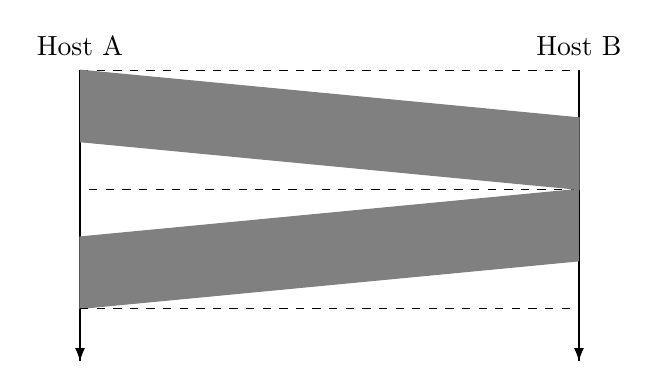
\begin{tikzpicture}
  
  \tikzstyle{every node}=[font=\normalsize]

  \tikzset{myptr/.style={decoration={markings,mark=at position 1
        with %
        {\arrow[black,scale=1.0,>=Latex]{>}}}, postaction={decorate}}}
  
  % Entities
  \node[] (Host A) {Host A};
  \node[right=5.0 of Host A] (Host B) {Host B};

  % Timelines
  \begin{pgfonlayer}{timelines}
    \coordinate (HA) at ($(Host A.center) + (0.0,-4.0)$);
    \draw[myptr] ($(Host A.center) + (0,-2ex)$) -- (HA);  
    \coordinate (HB) at ($(Host B.center) + (0.0,-4.0)$);
    \draw[myptr] ($(Host B.center) + (0,-2ex)$) -- (HB);
  \end{pgfonlayer}

  % Horizontal dashed line representing the same time in both timelines
  \coordinate (A sends first bit) at ($(Host A) + (0, -2ex)$);
  \coordinate (waiting for ping) at ($(Host B) + (0, -2ex)$);
  \draw[dashed] (A sends first bit) -- (waiting for ping);

  % Oblique line with the transmission of the first bit
  \coordinate (B receives first bit) at ($(Host B) + (0, -6ex)$);
  \coordinate (A sends last bit) at ($(Host A) + (0, -8ex)$);
  \coordinate (B receives last bit) at ($(Host B) + (0, -12ex)$);
  \filldraw[gray] (A sends first bit) -- (B receives first bit) -- (B receives last bit) -- (A sends last bit);

  % Second horizontal dashed line representing the same time in both timelines
  \coordinate (B receives last bit at A) at ($(Host A) + (0, -12ex)$);
  \draw[dashed] (B receives last bit) -- (B receives last bit at A);

  % Respose
  \coordinate (A receives first bit) at ($(Host A) + (0, -16ex)$);
  \coordinate (A receives last bit) at ($(Host A) + (0, -22ex)$);
  \coordinate (B sends last bit) at ($(Host B) + (0, -18ex)$);
  \filldraw[gray] (B receives last bit) -- (A receives first bit) -- (A receives last bit) -- (B sends last bit);

  % Second horizontal dashed line representing the same time in both timelines
  \coordinate (A receives last bit at B) at ($(Host B) + (0, -22ex)$);
  \draw[dashed] (A receives last bit) -- (A receives last bit at B);

  % RTT

\end{tikzpicture}

\end{document}
